% This text is proprietary.
% It's a part of presentation made by myself.
% It may not used commercial.
% The noncommercial use such as private and study is free
% May 2007
% Author: Sascha Frank 
% University Freiburg 
% www.informatik.uni-freiburg.de/~frank/
%
% 
\documentclass[]{beamer}
\usepackage{beamerthemeshadow}
%\setbeamertemplate{headline}{}
%\beamertemplatenavigationsymbolsempty
%\usepackage[]{media9}
\usepackage[flushleft]{threeparttable}
\usepackage{multimedia}
\usepackage{multirow}
%\usepackage{multibbl}
\usepackage{graphicx}
%\usepackage{cite}
\usepackage{array}
\usepackage{graphics}
\usepackage{multirow}
%\useoutertheme{infolines}
\usepackage{acronym}

%\newbibliography{main}
%\newbibliography{mypublications}

%%%%%%%%%%%%%%%%%%%%%%%%

\definecolor{recyellow}{rgb}{0.70,0.70,0.00}
\definecolor{cyan}{rgb}{0.00,1.00,1.00}
\definecolor{orange}{rgb}{1.00,0.50,0.00}
\definecolor{brown}{rgb}{0.70,0.20,0.20}
\definecolor{magenta}{rgb}{1.00,0.00,1.00}
\definecolor{black}{rgb}{0.00,0.00,0.00}
\definecolor{red}{rgb}{1.00,0.00,0.00}
\definecolor{blue}{rgb}{0.00,0.00,1.00}
\definecolor{green}{rgb}{0.4,1.00,0.0}
\definecolor{darkgreen}{rgb}{0.0,0.70,0.0}
\definecolor{yellow}{rgb}{0.5,0.5,0.0}
\definecolor{linkcolor1}{rgb}{0.0,0.0,0.5}
\definecolor{citecolor1}{rgb}{0.0,0.3,0.0}
\newcommand{\cred}[1] {\textcolor{red}{#1}}
\newcommand{\cblue}[1] {\textcolor{blue}{#1}}
\newcommand{\cgreen}[1] {\textcolor{green}{#1}}
\newcommand{\cdarkgreen}[1] {\textcolor{darkgreen}{#1}}
\newcommand{\cyellow}[1] {\textcolor{yellow}{#1}}
\newcommand{\crecyellow}[1] {\textcolor{recyellow}{#1}}
\newcommand{\ccyan}[1] {\textcolor{cyan}{#1}}
\newcommand{\cmagenta}[1] {\textcolor{magenta}{#1}}
\newcommand{\cbrown}[1] {\textcolor{brown}{#1}}
\newcommand{\corange}[1] {\textcolor{orange}{#1}}

\usepackage{hyperref}
\hypersetup{
   colorlinks=true,%
   citecolor=citecolor1,%
   filecolor=green,%
   linkcolor=linkcolor1,%
   urlcolor=green
}
%\bibliographystyle{ThesisStyleWithEtAl}
%\bibliography{bib/mypubs,bib/motionplanning,bib/colorcorrection,bib/inverseperspectivemapping,bib/roaddetection,bib/autonomous_vehicles,bib/softwarearchitecture,bib/polygonal_primitives,bib/photometric_scene_reconstruction,bib/officialdocs}{References}

%\usepackage{bibentry}
%\nobibliography *
%\let\newblock\relax


\setbeamertemplate{footline}[frame number]

\begin{document}

\title{ROS Workshop}  
\author{Miguel Oliveira, H\'{e}ber Sobreira}
%\institute{Universidade de Aveiro}
%\date{}

%% Title slide
\begin{frame}
\titlepage
\scriptsize CROB - Centro de Rob\'{o}tica e Sistemas Inteligentes \\
\scriptsize INESC TEC\\
\end{frame}

%%Table of contents
\begin{frame}\frametitle{Table of contents}
\scriptsize
\tableofcontents
\end{frame} 


\section{Objectives} 
\begin{frame}\frametitle{Objectives} 
\begin{itemize}
\item Lets play a game called \textbf{Team Hunt} (just made that up, don't
        bother googling)
\item Basic rules: 
\begin{itemize}
\item Three or more teams of one or more players
\item Players on a team hunt players from another team, while at the same
time they must evade players from a different other team
\begin{itemize}
    \item Ex. \textit{Team A} hunts \textit{Team B} hunts \textit{Team C} hunts \textit{Team A}
\end{itemize}
\item A player is killed if another player (from a team hunting him) gets close
enough (bellow a threshold)
\item The team which has hunted more players wins the game
\end{itemize}
\item The game takes place in an arena with fixed dimensions (in 2D)
\item Each player will have a turn to decide how to move.
\end{itemize}
\end{frame}

\section{What we will learn to do in ROS} 
\begin{frame}\frametitle{What we will learn to do in ROS} 
\begin{itemize}
\item Creating ROS packages, nodes and libraries, compiling and running them
\item Using ROS based communications, publish / subscribe, server / response
\item Using ROS launch file scripts to ease the startup of complex systems
\item Using ros parameters to configure the nodes
\item Creating custom messages
\item Using RVIZ and publishing visualization markers
\item Visualizing the ROS nodes and the topics they are exchanging
\item Using the ROS tf library (just the basics)
\item Using the rosbag tool to record the system's output
\item a lot more I don't remember right now \ldots
\end{itemize}
\end{frame}

\section{Prerequisites} 
\begin{frame}\frametitle{What must be done before starting the workshop}
\begin{itemize}
\item Install Ubuntu 14.04 64bit and ROS indigo 
\begin{itemize}
\item Other configurations are possible, but if something goes wrong we will not
have time to try to solve the problems
\end{itemize}
\item Tutorials 1 through 16 from \url{http://wiki.ros.org/ROS/Tutorials} should
be completed before starting the workshop
\begin{itemize}
\item use the catkin (and not rosbuild) to build your packages
\item you can skip the python tutorials
\end{itemize}
\item C++ tutorials at \url{http://www.cplusplus.com/doc/}, take a look if you
have no C++ background
\end{itemize}
\end{frame}

\section{System architecture} 
\begin{frame}\frametitle{Software architecture}
\begin{itemize}
\item The game runs in multiple processes, which communicate with each other
\item Each player is a process (a ros node), which will have the following interfaces: 
\begin{itemize}
\item Subscribe to a message (\textit{player\_move}) which will give the command to a
player to move
\item Broadcast a tf transform to let other players know about its position
\item Provide a service (\textit{kill\_me}), to be called by the hunters
\item Access a service (\textit{add\_points\_to\_team}) provided by the referee
\item Publish rviz markers to show his position in the arena, along with some
\textit{nasty comments} to intimidate the adversaries
\end{itemize}
\end{itemize}
\end{frame}

\section{Example} 
\begin{frame}\frametitle{Example}
\begin{figure}[!t] \scriptsize
\begin{center}
\centerline{
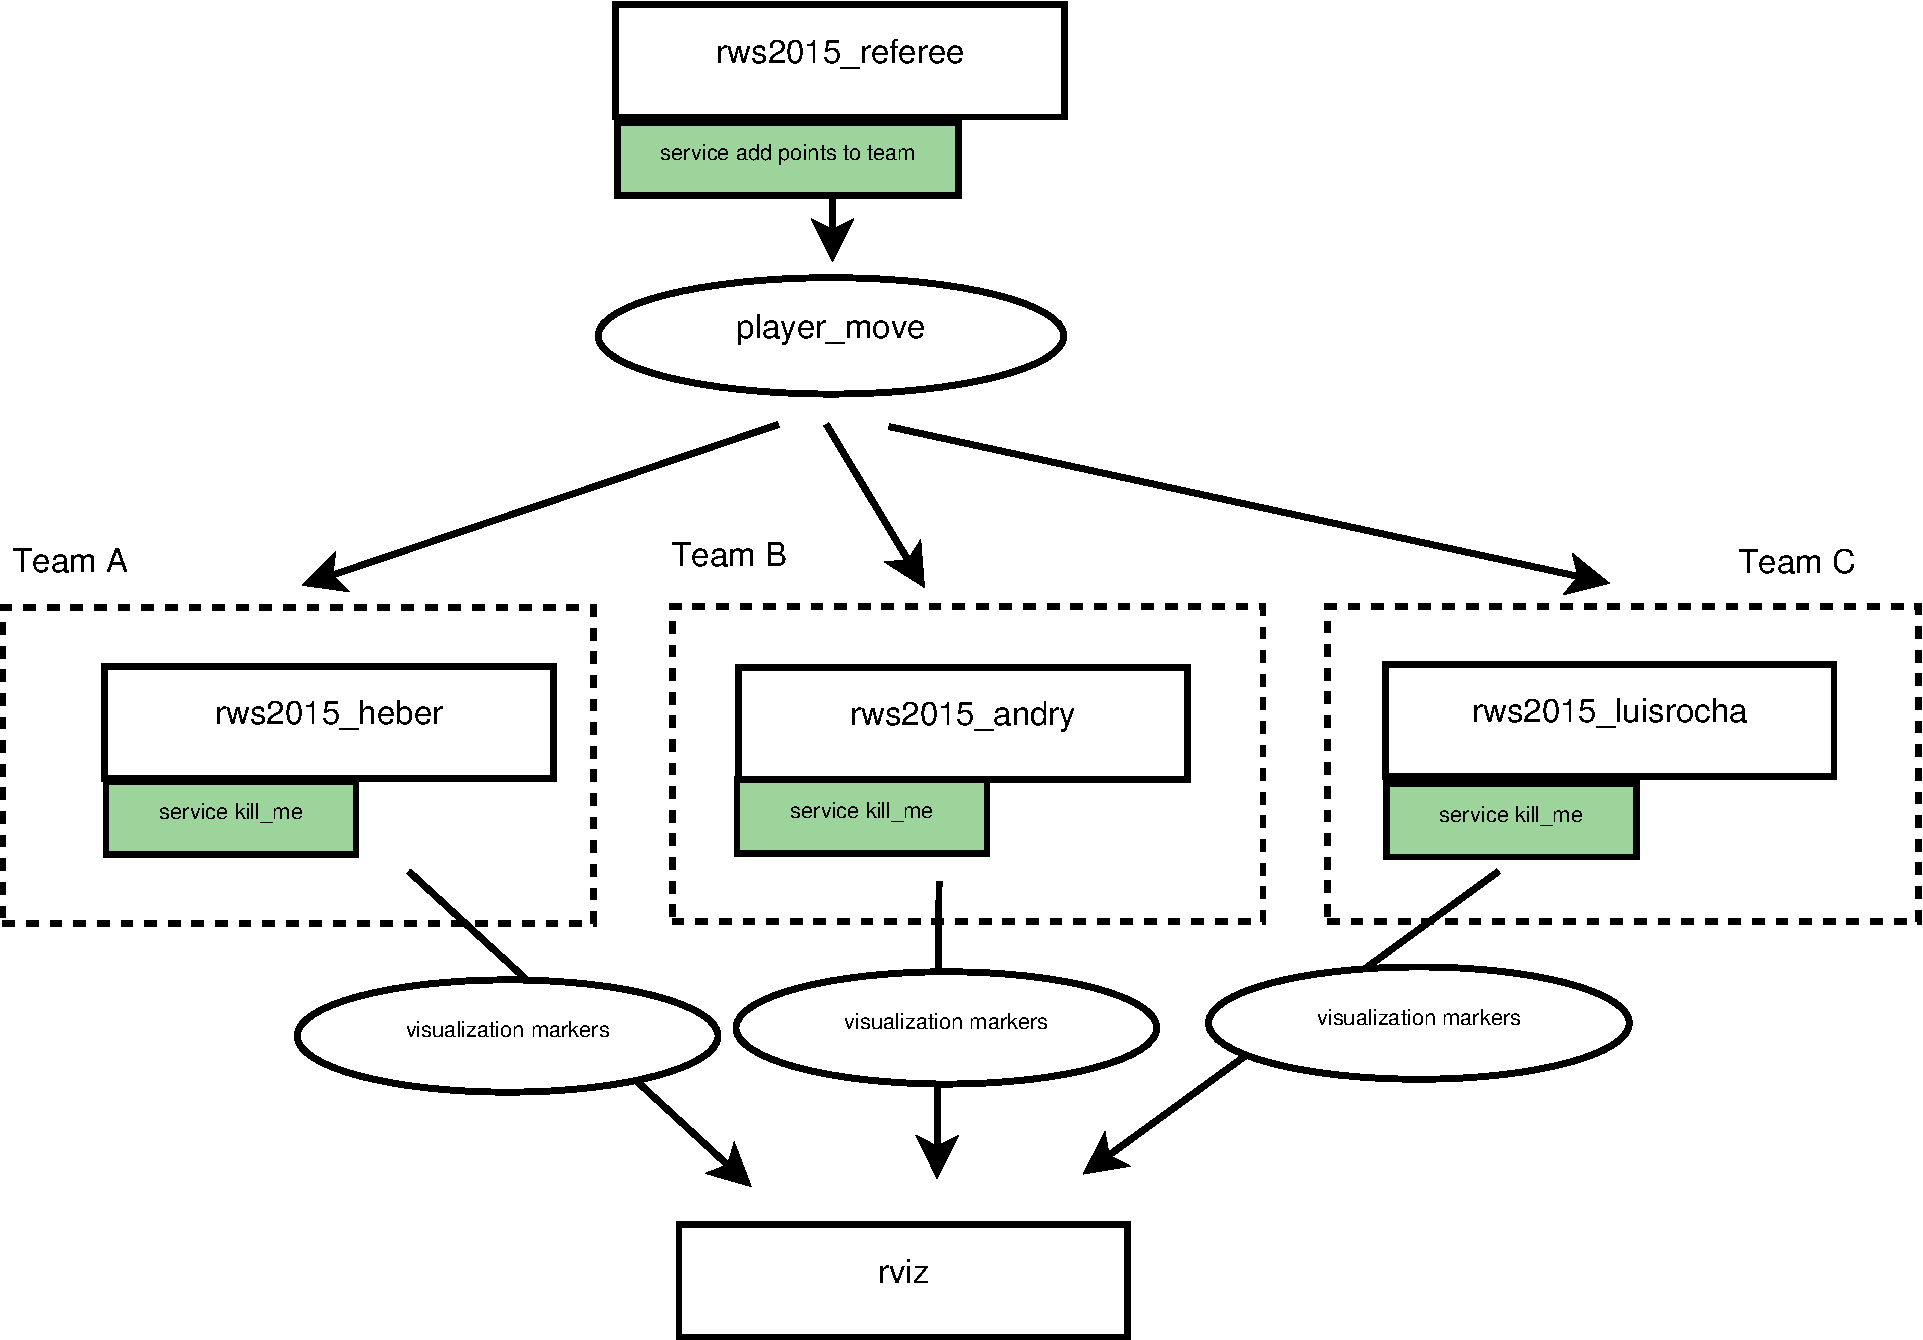
\includegraphics[width=.9\linewidth]{example.pdf}
}
\end{center}
\end{figure}
\end{frame}


%%%%%%%%%%%%%%%%%
%\begin{frame} \frametitle{Motivation and Objectives} 
%\begin{columns}
%\hspace{-25pt}
%\begin{column}{5cm}
%\begin{itemize}
%\small
%\item Technology onboard vehicles
%\item Positive impact
%\item Technologies at an early stage of development
%\item Global description of the scene
%\item High level understanding
%\item Asynchronous, large size, multi-modal data
%\end{itemize}
%\end{column}
%\begin{column}{5cm}
%\hspace{-15pt}
%\movie[height=0.5\textheight,width=0.8\textheight,showcontrols=true,poster,autoplay]{}{presentation/movies/i.wmv}
%\end{column}
%\end{columns}
%\pause
%\vspace{+10pt}
%\cred{Objective} to develop alternative data representations that may cope with multiple
%sensors and that improve the effectiveness of subsequent processing algorithms
%\end{frame}

%%%%%%%%%%%
%\begin{frame}[t]\frametitle{Contributions}
%\begin{columns}
%\begin{column}{0.8\textwidth}
%\begin{itemize}
%\small
%\item 3 Robot Prototypes
%\begin{itemize}
%\scriptsize
%\item Developed three robotic prototypes
%\item Autonomous Driving Competitions
%\end{itemize}
%\item 4 Software Architectures
%\begin{itemize}
%\scriptsize
%\item CARMEN, ROS and LARtk
%\end{itemize}
%\item 5 Inverse Perspective Mapping
%\begin{itemize}
%\scriptsize
%\item Proposed a multi-modal, multi-camera IPM
%\end{itemize}
%\item 6 Photometric Calibration
%\begin{itemize}
%\scriptsize
%\item Proposed three approaches for color correction
%\end{itemize}
%\vspace{+4pt}
%\item 7 Datasets and Preprocessing
%\vspace{+9pt}
%\item 8-9 Geometric Reconstruction and Refinement
%\vspace{+2pt}
%\item 10-11 Photometric Reconstruction and Refinement
%\end{itemize}
%\end{column}
%\begin{column}[t]{0.2\textwidth}
%\vspace{-95pt}
%\begin{center}
%\includegraphics[width=0.7\linewidth]{chapters/multisensor_data_representation/Figures/atlascar1.pdf}\\
%\vspace{+5pt}
%\includegraphics[width=1\linewidth]{chapters/software_architectures/Figures/control.pdf}\\
%\vspace{+2pt}
%\includegraphics[width=0.9\linewidth]{chapters/multisensor_data_representation/Figures/road_figure1_caption.pdf}\\
%\vspace{+2pt}
%\includegraphics[width=0.5\linewidth]{chapters/photometric_registration/Figures/regiondefinition2.pdf}\\
%\vspace{+2pt}
%\includegraphics[width=0.5\linewidth]{chapters/polygonal_primitives/Figures/mit/seq1/path.pdf}\\
%\vspace{+2pt}
%\includegraphics[width=0.8\linewidth,clip=true, trim=0 100 0 200]{chapters/polygonal_primitives/Figures/geometricpp/ex1_3d.pdf}\\
%\vspace{+2pt}
%\includegraphics[width=0.9\linewidth,clip=true, trim=0 0 0 0]{chapters/photometric_scene_reconstruction/Figures/tm_results/cam_fc6mm_tm.pdf}\\
%\end{center}
%\end{column}
%\end{columns}
%\end{frame}

%%%%%%%%%%%
%\begin{frame}[t]\frametitle{Contributions}
%\begin{columns}
%\begin{column}{0.8\textwidth}
%\begin{itemize}
%\small
%\item 3 Robot Prototypes
%\begin{itemize}
%\scriptsize
%\item Developed three robotic prototypes
%\item Autonomous Driving Competitions
%\end{itemize}
%\item 4 Software Architectures
%\begin{itemize}
%\scriptsize
%\item CARMEN, ROS and LARtk
%\end{itemize}
%\item 5 Inverse Perspective Mapping
%\begin{itemize}
%\scriptsize
%\item Proposed a multi-modal, multi-camera IPM
%\end{itemize}
%\item 6 Photometric Calibration
%\begin{itemize}
%\scriptsize
%\item Proposed three approaches for color correction
%\end{itemize}
%\vspace{+4pt}
%\item 7 Datasets and Preprocessing
%\vspace{+9pt}
%\item \underline{8-9 Geometric Reconstruction and Refinement}
%\vspace{+2pt}
%\item \underline{10-11 Photometric Reconstruction and Refinement}
%\end{itemize}
%\end{column}
%\begin{column}[t]{0.2\textwidth}
%\vspace{-95pt}
%\begin{center}
%\includegraphics[width=0.7\linewidth]{chapters/multisensor_data_representation/Figures/atlascar1.pdf}\\
%\vspace{+5pt}
%\includegraphics[width=1\linewidth]{chapters/software_architectures/Figures/control.pdf}\\
%\vspace{+2pt}
%\includegraphics[width=0.9\linewidth]{chapters/multisensor_data_representation/Figures/road_figure1_caption.pdf}\\
%\vspace{+2pt}
%\includegraphics[width=0.5\linewidth]{chapters/photometric_registration/Figures/regiondefinition2.pdf}\\
%\vspace{+2pt}
%\includegraphics[width=0.5\linewidth]{chapters/polygonal_primitives/Figures/mit/seq1/path.pdf}\\
%\vspace{+2pt}
%\includegraphics[width=0.8\linewidth,clip=true, trim=0 100 0 200]{chapters/polygonal_primitives/Figures/geometricpp/ex1_3d.pdf}\\
%\vspace{+2pt}
%\includegraphics[width=0.9\linewidth,clip=true, trim=0 0 0 0]{chapters/photometric_scene_reconstruction/Figures/tm_results/cam_fc6mm_tm.pdf}\\
%\end{center}
%\end{column}
%\end{columns}
%\end{frame}

%%%%%%%%%%%%%%%%%%
%%\begin{frame} \frametitle{Atlas Project} 
%%\begin{figure}[ht]
%%%%\movie[poster,autoplay,externalviewer,text={\small(Loading
%%%%Video...)}]{mov1.avi}
%%\movie[height=0.1\textheight,width=0.1\textheight,showcontrols=true,poster,autoplay]{}{presentation/movies/i.avi}
%%\end{figure}

%%\begin{columns}
%%\begin{column}{5cm}
%%\begin{itemize}
%%\item  
%%\end{itemize}
%%\end{column}
%%\begin{column}{5cm}
%%\end{column}
%%\end{columns}
%%\end{frame}


%%%%%%%%%%%%
%\section{Geometric Scene Reconstruction}

%\subsection{Introduction}

%%%%%%%%%
%\begin{frame}\frametitle{Scene Reconstruction}
%\begin{itemize}
%\item The computation of a (textured) geometric 3D model
%\pause
%\item Range (and photometric) measurements 
%\pause
%\item To compute an alternative representation of the environment
%\begin{itemize}
%\item \cred{Continuous}
%\item \cred{Unique}
%\item \cred{Efficient}
%\pause
%\end{itemize}
%\end{itemize}
%\begin{columns}
%\begin{column}{10cm}
%\begin{itemize}
%\item Surface description representations
%\begin{itemize}
%\item 3D Delaunay triangulations, \textbf{BPA} or Poisson
%\item Noisy measurements, nearest neighbor queries
%\item Computer graphics
%\pause
%\end{itemize}
%\item Volumetric occupancy representations
%\begin{itemize}
%\item Occupancy grids, (extended) elevation maps or octrees
%\item inaccurate geometric information, no texture mapping
%\item Robotics
%\end{itemize}
%\end{itemize}
%\end{column}
%\hspace{-45pt}
%\begin{column}{5cm}
%\begin{figure}[!t] 
%\begin{center}
%\centerline{
%\begin{tabular}{c}
%\includegraphics[width=0.3\linewidth]{presentation/images/bunny_tri.pdf}\\
%\includegraphics[width=0.3\linewidth]{presentation/images/bunny.pdf}\\
%\end{tabular}
%}\end{center}
%\end{figure}
%\end{column}
%\end{columns}
%\end{frame}

%%%%%%%%%
%\begin{frame}\frametitle{Scene Reconstruction}
%\begin{itemize}
%\item The computation of a (textured) geometric 3D model
%\item Range (and photometric) measurements 
%\item To compute an alternative representation of the environment
%\begin{itemize}
%\item \cred{Continuous}
%\item \cred{Unique}
%\item \cred{Efficient}
%\end{itemize}
%\end{itemize}
%\begin{columns}
%\begin{column}{10cm}
%\begin{itemize}
%\item \underline{Surface description representations}
%\begin{itemize}
%\item 3D Delaunay triangulations, \textbf{BPA} or Poisson
%\item Noisy measurements, nearest neighbor queries
%\item Computer graphics
%\end{itemize}
%\item Volumetric occupancy representations
%\begin{itemize}
%\item Occupancy grids, (extended) elevation maps or octrees
%\item inaccurate geometric information, no texture mapping
%\item Robotics
%\end{itemize}
%\end{itemize}
%\end{column}
%\hspace{-45pt}
%\begin{column}{5cm}
%\begin{figure}[!t] 
%\begin{center}
%\centerline{
%\begin{tabular}{c}
%\includegraphics[width=0.3\linewidth]{presentation/images/bunny_tri.pdf}\\
%\includegraphics[width=0.3\linewidth]{presentation/images/bunny.pdf}\\
%\end{tabular}
%}\end{center}
%\end{figure}
%\end{column}
%\end{columns}
%\end{frame}

%%%%%%%%%%%
%\begin{frame}\frametitle{MIT DARPA Urban Challenge dataset}\scriptsize
%\begin{figure}[!t] \scriptsize
%\begin{center}
%\centerline{
%\begin{tabular}{c}
%\includegraphics[width=0.7\linewidth]{chapters/polygonal_primitives/Figures/mit/seq1/path.pdf}\\
%\end{tabular}
%}\end{center}
%\vspace{-15pt}
%\end{figure}
%\scriptsize Path travelled by the robot during sequence 1. Key locations are
%annotated both in the map and the zoomed in image\\
%\cred{Location \emph{C}} will be used as case study
%\end{frame}

%%%%%%%%%%%
%\begin{frame}\frametitle{Raw data captured by the vehicle}\scriptsize
%\begin{figure}[!b]
%\begin{center}
%\centerline{
%\begin{tabular}{ccc}
%\multicolumn{2}{c}{\includegraphics[width=0.7\linewidth]{chapters/polygonal_primitives/Figures/mit/seq1/scnC_iso.pdf}} &
%\includegraphics[width=0.21\linewidth]{chapters/polygonal_primitives/Figures/mit/seq1/scnC_fc6mm.pdf}\\
%\includegraphics[width=0.20\linewidth]{chapters/polygonal_primitives/Figures/mit/seq1/scnC_top.pdf}&
%\includegraphics[width=0.16\linewidth]{chapters/polygonal_primitives/Figures/mit/seq1/scnC_map.pdf}&
%\includegraphics[width=0.21\linewidth]{chapters/polygonal_primitives/Figures/mit/seq1/scnC_fc.pdf}\\
%\includegraphics[width=0.21\linewidth]{chapters/polygonal_primitives/Figures/mit/seq1/scnC_fl.pdf}&
%\includegraphics[width=0.21\linewidth]{chapters/polygonal_primitives/Figures/mit/seq1/scnC_fr.pdf}&
%\includegraphics[width=0.21\linewidth]{chapters/polygonal_primitives/Figures/mit/seq1/scnC_rc.pdf}\\
%\end{tabular}
%}\end{center}
%\label{fig:seq1_scnC_example}
%\vspace{-10pt}
%\end{figure}
%Raw data acquired by the vehicle at \cred{location \emph{C}} of the sequence 1 
%\end{frame}

%%%%%%%%%%%
%\begin{frame}\frametitle{Sequence 1 raw data}
%\begin{center}
%\movie[height=0.8\textheight,width=1.2\textheight,autostart,showcontrols=true]{}{presentation/movies/seq1.ogv}
%\end{center}
%\scriptsize Only the latest \textit{Velodyne} scan is shown
%\end{frame}

%%%%%%%%%%%
%\begin{frame}\frametitle{Continuity}
%\begin{center}
%\movie[height=0.8\textheight,width=1.2\textheight,autostart,showcontrols=true]{}{presentation/movies/continuity.ogv}
%\end{center}
%\scriptsize Range measurements are always a discretized view of the environment
%\end{frame}

%%%%%%%%%%%
%\begin{frame}\frametitle{Uniqueness}
%\begin{center}
%\movie[height=0.8\textheight,width=1.2\textheight,autostart,showcontrols=true]{}{presentation/movies/multiplemeasurements.ogv}
%\end{center}
%\scriptsize Over time, there are multiple measurements of the same surfaces
%\end{frame}

%%%%%%%%%%%
%\begin{frame}\frametitle{Memory efficiency}\scriptsize
%pt, number of points; size, memory
%size (MB); t, mission time (secs); d, traveled distance (meters)
%\begin{table}[!b]\footnotesize
%\begin{center}
%\label{table:infolocationseq1}
%\vspace{-15pt}
%\begin{tabular}{|c|c|c|c|c|c|c|}
%\hline
 %\multicolumn{1}{|c|}{Location}& \multicolumn{2}{c|}{Location Snapshot} &
 %\multicolumn{4}{c|}{Sequence accumulated} \\
%\hline
%Name &  pt $(\times10^6)$ & size (MB) & pt $(\times10^6)$&
%size (MB) & t (s)& d (m)\\
%\hline 
%\emph{A} & 1.3 & 15.6 & 
%1.3 & 15.6 & 1 & 0\\
%\emph{B} & 1.3 & 15.6 &
%13.0 & 156.0 & 11 & 75\\
%\cred{\emph{C}} & \cred{1.3} & \cred{15.6} & 
%\cred{26.0} &\cred{312.0} &\cred{21} &\cred{125}\\
%\emph{D} & 1.3 & 15.6 & 
%39.0 & 468.0  & 31 & 140\\
%\emph{E} & 1.3 & 15.6 &
%52.0 & 624.0 & 41 & 190\\
%\hline
%\end{tabular}
%\end{center}
%\end{table}
%\end{frame}

%%%%%%%%%%%
%\begin{frame}\frametitle{Compression using Preprocessing} \scriptsize
%\begin{figure}[!t]
%\begin{center}
%\centerline{
%\begin{tabular}{c}
%\includegraphics[width=0.7\linewidth]{chapters/polygonal_primitives/Figures/preprocessingseq1_graph.pdf}
%\end{tabular}
%}\end{center}
%\vspace{-15pt}
%\label{fig:fullfilter_graph}
%\end{figure}
%\scriptsize Size of the accumulated point clouds using raw (\cred{red}) and
%preprocessed data (\cblue{blue}) as a function of the mission time 
%\end{frame}

%%%%%%%%%%%
%\subsection{Proposed Approach}

%%%%%%%%%%%
%\begin{frame}\frametitle{Geometric scene reconstruction}
%\begin{itemize}
%\item Use a surface based representation
%\pause
%\item Basic elements are polygons, as opposed to triangles
%\pause
%\end{itemize}
%\begin{figure}[!t]
%\begin{center}
%\centerline{
%\begin{tabular}{cc}
%\includegraphics[width=0.35\linewidth]{chapters/polygonal_primitives/Figures/geometricpp/ex1_fc.pdf}&
	%\vspace{-20pt}
%\includegraphics[width=0.35\linewidth]{chapters/polygonal_primitives/Figures/geometricpp/ex1_fc6mm.pdf}\\
%\multicolumn{2}{c}{\includegraphics[width=0.8\linewidth]{chapters/polygonal_primitives/Figures/geometricpp/ex1_3d.pdf}}\\ 
%\end{tabular}
%}\end{center}
%\label{fig:geometricpp1}
%\end{figure}
%\end{frame}

%%%%%%%%%%%
%\begin{frame}[t]\frametitle{RANSAC}
%\begin{itemize}
%\item \small STEP 1 - Detect candidate polygonal primitives using RANSAC
%\end{itemize}
%\begin{figure}[!t]
%\begin{center}
%\centerline{
%\begin{tabular}{cc}
%\includegraphics[width=0.52\linewidth]{chapters/polygonal_primitives/Figures/geometricpp/ransac_mt1_1_detail.pdf}&
%\includegraphics[width=0.52\linewidth]{chapters/polygonal_primitives/Figures/geometricpp/ransac_mt1_2.pdf}\\
%\includegraphics[width=0.52\linewidth]{chapters/polygonal_primitives/Figures/geometricpp/ransac_mt2_1.pdf}&
%\includegraphics[width=0.52\linewidth]{chapters/polygonal_primitives/Figures/geometricpp/ransac_mt2_2.pdf}\\
%\end{tabular}
%}\end{center}
%\label{fig:geometricpp2}
%\end{figure}
%\end{frame}

%%%%%%%%%%%
%\begin{frame}[t]\frametitle{Clustering}
%\begin{itemize}
%\item \small STEP 2 - Cluster RANSAC inliers
%\end{itemize}
%\begin{figure}[!t]
%\begin{center}
%\centerline{
%\begin{tabular}{c}
%\includegraphics[width=0.8\linewidth,clip=true, trim=0 0 0 80]{chapters/polygonal_primitives/Figures/geometricpp/cluster_bad.pdf}\\
%\includegraphics[width=0.8\linewidth,clip=true, trim=0 0 0 80]{chapters/polygonal_primitives/Figures/geometricpp/cluster_good.pdf}\\
%\end{tabular}
%}\end{center}
%\label{fig:geometricpp5a}
%\end{figure}
%\end{frame}

%%%%%%%%%%%
%\begin{frame}[t]\frametitle{Plane Estimation}
%\begin{itemize}
%\item \small STEP 3 - Reestimate plane coefficients using PCA
%\end{itemize}
%\begin{figure}[!t]
%\begin{center}
%\centerline{
%\begin{tabular}{c}
%\begin{tabular}{cc}
%\includegraphics[width=0.7\linewidth]{chapters/polygonal_primitives/Figures/geometricpp/pca3.pdf}&
%\includegraphics[width=0.19\linewidth]{chapters/polygonal_primitives/Figures/geometricpp/pca4.pdf}\\
%\end{tabular}
%\end{tabular}
%}\end{center}
%\label{fig:geometricpp4}
%\end{figure}
%\end{frame}

%%%%%%%%%%%
%\begin{frame}[t]\frametitle{Compute bounding polygon}
%\begin{itemize}
%\item \small STEP 4 - Compute bounding polygon 
%\end{itemize}
%\begin{figure}[!t]
%\begin{center}
%\centerline{
%\begin{tabular}{cc}
%\includegraphics[width=0.48\linewidth]{chapters/polygonal_primitives/Figures/geometricpp/polygon3.pdf}&
%\includegraphics[width=0.48\linewidth]{chapters/polygonal_primitives/Figures/geometricpp/polygon4.pdf}\\
%\end{tabular}
%}\end{center}
%\label{fig:geometricpp5}
%\end{figure}
%\scriptsize Convex hull (\cblue{blue}), concave hull (\cred{red})
%\end{frame}

%%%%%%%%%%%
%\subsection{Results}

%%%%%%%%%%%
%\begin{frame}[t]\frametitle{Processing time}
%\begin{table}[!b] \footnotesize
%\begin{center}
%\label{table:comparisson_computation_time}
%\begin{tabular}{|c|c|c|c|c|c|c|}
%\hline
%& \multicolumn{5}{c|}{Processing time (secs)}\\
%Location & \textbf{BPA}&\textbf{GT}& \textbf{POIS}&
%\textbf{GPP}1& \textbf{GPP}2\\
%\hline
%\scriptsize
%\emph{A} &659.0 &154.0	& 63.2 & 16.3& 27.3\\
%\emph{B} &752.9 &157.5	& 61.6& 25.3 & 17.4\\
%\cred{\emph{C}} & \cred{488.2} &\cred{156.3}& \cred{56.3}& \cred{13.5}&\cred{49.4}\\
%\emph{D} &480.4 &142.4	& 52.6& 25.2 & 25.2\\
%\emph{E} &558.8 &149.0	& 57.9& 47.4 & 58.1\\
%\hline
%$\mu$ & 585.9&151.8  & 58.3& 25.5 &35.5\\
%\hline
%\end{tabular}
%\end{center}
%\end{table}
%\pause
%\begin{itemize}
%\item \textbf{GPP}1 \underline{2 times} faster than \textbf{POIS}
%\item \textbf{GPP}1 \underline{6 times} faster than fastest 3D triangulation (\textbf{GT})
%\end{itemize}
%\end{frame}

%%%%%%%%%%%
%\begin{frame}[t]\frametitle{Processing time}
%\begin{table}[!b] \footnotesize
%\begin{center}
%\label{table:comparisson_computation_time}
%\begin{tabular}{|c|c|c|c|c|c|c|}
%\hline
%& \multicolumn{5}{c|}{Processing time (secs)}\\
%Location & \cblue{\textbf{BPA}}&\textbf{GT}& \textbf{POIS}&
%\cdarkgreen{\textbf{GPP}1}& \cdarkgreen{\textbf{GPP}2}\\
%\hline
%\scriptsize
%\emph{A} &\cblue{659.0} &154.0	& 63.2 & 16.3& 27.3\\
%\emph{B} &\cblue{752.9} &157.5	& 61.6& 25.3 & 17.4\\
%\cred{\emph{C}} & \cblue{488.2} &\cred{156.3}& \cred{56.3}& \cred{13.5}&\cred{49.4}\\
%\emph{D} &\cblue{480.4} &142.4	& 52.6& 25.2 & 25.2\\
%\emph{E} &\cblue{558.8} &149.0	& 57.9& 47.4 & 58.1\\
%\hline
%$\mu$ & \cblue{585.9}&151.8  & 58.3& 25.5 &35.5\\
%\hline
%\end{tabular}
%\end{center}
%\end{table}
%\begin{itemize}
%\item \textbf{GPP}1 \underline{2 times} faster than \textbf{POIS}
%\item \textbf{GPP}1 \underline{6 times} faster than fastest 3D triangulation (\textbf{GT})
%\item \cblue{\textbf{BPA} is used as ground truth for measuring accuracy}
%\end{itemize}
%\end{frame}

%%%%%%%%%%%
%\begin{frame}\frametitle{Accuracy}
%\begin{table}[!b] \scriptsize
%\begin{center}
%\label{table:comparisson_accuracy}
%\begin{tabular}{|c|ccc|ccc|ccc|}
%\hline
%& \multicolumn{9}{c|}{Hausdorff distance (meters)}\\
%Location & \multicolumn{3}{c|}{\textbf{GT}} &\multicolumn{3}{c|}{\textbf{POIS}}
%&\multicolumn{3}{c|}{\cdarkgreen{\textbf{GPP} 1}} \\
 %& max & mean & RMS &  max & mean & RMS &max & mean & RMS \\
%\hline
%\emph{A} & 11.7 & 0.15 & 0.41 & 14.0 & 1.39 & 2.98&7.6&1.02&1.71\\
%\emph{B} & 11.8 & 0.12 & 0.37 & 14.1 & 1.39 & 2.99&12.7& 0.94&1.77\\
%\cred{\emph{C}} & \cred{12.7} & \cred{0.18} & \cred{0.44} & \cred{13.9} &\cred{1.06} & \cred{2.59}& \cred{8.9}&\cred{0.87}&\cred{1.54}\\
%\emph{D} & 13.8 & 0.10 & 0.40 & 13.9 & 1.90 & 4.00 & 7.6&0.86&1.47\\
%\emph{E} & 12.5 & 0.14 & 0.49 & 14.0 & 1.42 & 3.03&14.0&1.25&2.56\\
%\hline
%$\mu$& 12.5 & 0.14 & 0.42 & 13.9 & 1.43 & 3.12&10.2&\cblue{0.99}&1.81\\
%\hline
%\end{tabular}
%\end{center}
%\end{table}
%\begin{itemize}
%\item 0.99 $\simeq$ 1 meter average error seems to be very large
%\item However ...
%\end{itemize}
%\end{frame}


%%%%%%%%%%%
%\begin{frame}[t]\frametitle{Accuracy}
%\begin{figure}[!t]
%\begin{center}
%\centerline{
%\begin{tabular}{cc}
%Ground truth (\textbf{BPA}) & \textbf{GPP}1\\
%\includegraphics[width=0.5\linewidth]{chapters/polygonal_primitives/Figures/geometricpp/comparison/hausdorff/location_E_set2_groundtruth.pdf}&
%\includegraphics[width=0.5\linewidth]{chapters/polygonal_primitives/Figures/geometricpp/comparison/hausdorff/location_E_set2_plg.pdf}\\
%\end{tabular}
%}\end{center}
%\label{fig:hausdorff_error}
%\end{figure}
%\end{frame}

%%%%%%%%%%%
%\begin{frame}[t]\frametitle{Accuracy}
%\begin{figure}[!t]
%\begin{center}
%\centerline{
%\begin{tabular}{cc}
%Ground truth (\textbf{BPA}) & \textbf{GPP}1\\
%\includegraphics[width=0.5\linewidth]{chapters/polygonal_primitives/Figures/geometricpp/comparison/hausdorff/location_E_set2_groundtruth.pdf}&
%\includegraphics[width=0.5\linewidth]{chapters/polygonal_primitives/Figures/geometricpp/comparison/hausdorff/location_E_set2_sample.pdf}\\
%\end{tabular}
%}\end{center}
%\label{fig:hausdorff_error}
%\end{figure}
%\begin{itemize}
%\item Zero error (\cred{red}), medium error (\cgreen{green}), large error (\cblue{blue})
%\end{itemize}
%\end{frame}

%%%%%%%%%%%
%\begin{frame}[t]\frametitle{Accuracy}
%\begin{figure}[!t]
%\begin{center}
%\centerline{
%\begin{tabular}{cc}
%Ground truth (\textbf{BPA}) & \textbf{GPP}1\\
%\includegraphics[width=0.5\linewidth]{chapters/polygonal_primitives/Figures/geometricpp/comparison/hausdorff/location_E_set2_groundtruth.pdf}&
%\includegraphics[width=0.5\linewidth]{chapters/polygonal_primitives/Figures/geometricpp/comparison/hausdorff/location_E_set2_noground_sample.pdf}\\
%\end{tabular}
%}\end{center}
%\label{fig:hausdorff_error}
%\end{figure}
%\begin{itemize}
%\item Zero error (\cred{red}), medium error (\cgreen{green}), large error (\cblue{blue})
%\item Use \underline{concave hull} and ground plane \underline{not included}
%\end{itemize}
%\end{frame}

%%%%%%%%%%%
%\begin{frame}[t]\frametitle{Accuracy}
%\begin{table}[!t] \scriptsize
%\begin{center}
%\label{table:comparisson_accuracy_gpp2}
%\begin{tabular}{|c|cc|cc|cc|cc|}
%\hline
%\scriptsize
%& \multicolumn{8}{c|}{\textbf{GPP} 2 Hausdorff distance (meters)}\\
%B. Polygon&\multicolumn{2}{c|}{Convex}&
%\multicolumn{2}{c|}{Convex}&\multicolumn{2}{c|}{Concave}&\multicolumn{2}{c|}{\underline{Concave}} \\
%Ground plane&\multicolumn{2}{c|}{Included}& \multicolumn{2}{c|}{Not	included}&\multicolumn{2}{c|}{Included}&\multicolumn{2}{c|}{\underline{Not included}} \\
 %& max & mean &  max & mean &max & mean &max & mean  \\
%\hline
%\emph{A} & 7.6&0.87&1.8&0.15&6.8&0.71&1.2&0.13\\
%\emph{B} & 12.6&0.81&1.5&0.11&12.6&0.53&1.1&0.08\\
%\cred{\emph{C}} & \cred{8.9}&\cred{0.69}&\cred{1.9}&\cred{0.16}&\cred{6.6}&\cred{0.52}&\cred{1.9}&\cred{0.12}\\
%\emph{D} & 7.6&0.69&2.2&0.14&7.3&0.59&2.1&0.11\\
%\emph{E} & 14.0&1.11&1.7&0.10&8.8&0.32&1.4&0.08\\
%\hline
%$\mu$& 10.1&0.83&1.8&0.13&8.4&0.53&1.5&\cblue{0.10}\\
%\hline
%\end{tabular}
%\end{center}
%\end{table}
%\begin{itemize}
%\item \cblue{0.10} average error better than all others
%\item \textbf{GT} had 0.14 average error
%\end{itemize}
%\end{frame}

%%%%%%%%%%%
%\begin{frame}\frametitle{Qualitative results}
%\begin{center}
%\movie[height=0.8\textheight,width=1.2\textheight,autostart,showcontrols=true]{}{presentation/movies/geometric_results.ogv}
%\end{center}
%\end{frame}


%%%%%%%%%%%%
%\section{Geometric scene refinement}

%%%%%%%%%%%%
%\subsection{Introduction}

%\begin{frame}\frametitle{Geometric scene refinement}
%\begin{itemize}
%\item How to handle repeated measurements of the same surface?
%\end{itemize}
%\begin{figure}[!t]
%\vspace{-20pt}
%\begin{center}
%\centerline{
%\begin{tabular}{cc}
%\vspace{-3pt}
%\scriptsize \textbf{BPA} & \scriptsize \hspace{-50pt} \textbf{GPP}\\
%\hspace{+20pt}
%\includegraphics[width=0.6\linewidth]{chapters/polygonal_primitives/Figures/refinegeometric/reconstruct/bpa01.pdf}&
%\hspace{-50pt}
%\includegraphics[width=0.6\linewidth]{chapters/polygonal_primitives/Figures/refinegeometric/reconstruct/gpp03.pdf}\\
%\end{tabular}
%}\end{center}
%\vspace{-10pt}
%\end{figure}
%\scriptsize Color notation: reconstruction at locations
%\crecyellow{A}, \cred{B}, \cgreen{C}, \cblue{D} and \ccyan{E}
%\pause
%\begin{itemize}
%\normalsize
%\item GPP expansion mechanism
%\begin{itemize}
%\scriptsize
%\item Faster than (re) detection
%\item Save computation time for the detection of novel data
%\end{itemize}
%\end{itemize}
%\end{frame}

%%%%%%%%%%%%
%\subsection{Proposed approach}

%\begin{frame}\frametitle{Perpendicular expansion}
%\begin{itemize}
%\item STEP 1: to find points have a smaller than \textit{T} perpendicular distance to the GPP's
%support plane
%\end{itemize}
%\begin{figure}[!t]
%\begin{center}
%\centerline{
%\begin{tabular}{cc}
%\includegraphics[width=0.5\linewidth]{chapters/polygonal_primitives/Figures/refinegeometric/expansion/perpendicular_threshold.pdf}&
%\includegraphics[width=0.5\linewidth]{chapters/polygonal_primitives/Figures/refinegeometric/expansion/perpendicular_threshold1.pdf}\\
%\end{tabular}
%}\end{center}
%\label{fig:expansion0}
%\end{figure}
%\end{frame}

%\begin{frame}\frametitle{Longitudinal expansion}
%\begin{itemize}
%\item STEP 2: Expand the bounding polygon iteratively 
%\item Initial situation
%\end{itemize}
%\begin{figure}[!t]
%\begin{center}
%\centerline{
%\begin{tabular}{c}
%\includegraphics[width=0.68\linewidth]{chapters/polygonal_primitives/Figures/refinegeometric/expansion/ex1.pdf}\\
%\end{tabular}
%}\end{center}
%\label{fig:expansion1}
%\end{figure}
%\end{frame}

%\begin{frame}\frametitle{Longitudinal expansion}
%\begin{itemize}
%\item STEP 2: Expand the bounding polygon iteratively 
%\item Iteration 1
%\end{itemize}
%\begin{figure}[!t]
%\begin{center}
%\centerline{
%\begin{tabular}{c}
%\includegraphics[width=0.68\linewidth]{chapters/polygonal_primitives/Figures/refinegeometric/expansion/ex2.pdf}\\
%\end{tabular}
%}\end{center}
%\label{fig:expansion1}
%\end{figure}
%\end{frame}

%\begin{frame}\frametitle{Longitudinal expansion}
%\begin{itemize}
%\item STEP 2: Expand the bounding polygon iteratively 
%\item Iteration 2
%\end{itemize}
%\begin{figure}[!t]
%\begin{center}
%\centerline{
%\begin{tabular}{c}
%\includegraphics[width=0.68\linewidth]{chapters/polygonal_primitives/Figures/refinegeometric/expansion/ex3.pdf}\\
%\end{tabular}
%}\end{center}
%\label{fig:expansion1}
%\end{figure}
%\end{frame}

%\begin{frame}\frametitle{Longitudinal expansion}
%\begin{itemize}
%\item STEP 2: Expand the bounding polygon iteratively 
%\item Iteration 3
%\end{itemize}
%\begin{figure}[!t]
%\begin{center}
%\centerline{
%\begin{tabular}{c}
%\includegraphics[width=0.68\linewidth]{chapters/polygonal_primitives/Figures/refinegeometric/expansion/ex4.pdf}\\
%\end{tabular}
%}\end{center}
%\label{fig:expansion1}
%\end{figure}
%\end{frame}

%\begin{frame}\frametitle{Longitudinal expansion}
%\begin{itemize}
%\item STEP 2: Expand the bounding polygon iteratively 
%\item Iteration 4
%\end{itemize}
%\begin{figure}[!t]
%\begin{center}
%\centerline{
%\begin{tabular}{c}
%\includegraphics[width=0.68\linewidth]{chapters/polygonal_primitives/Figures/refinegeometric/expansion/ex5.pdf}\\
%\end{tabular}
%}\end{center}
%\label{fig:expansion1}
%\end{figure}
%\end{frame}

%\begin{frame}\frametitle{Longitudinal expansion}
%\begin{itemize}
%\item STEP 2: Expand the bounding polygon iteratively 
%\item Iteration 5
%\end{itemize}
%\begin{figure}[!t]
%\begin{center}
%\centerline{
%\begin{tabular}{c}
%\includegraphics[width=0.68\linewidth]{chapters/polygonal_primitives/Figures/refinegeometric/expansion/ex6.pdf}\\
%\end{tabular}
%}\end{center}
%\label{fig:expansion1}
%\end{figure}
%\end{frame}

%%%%%%%%%%%%
%\subsection{Results}

%%%%%%%%%%%
%\begin{frame}\frametitle{Qualitative results}
%\begin{center}
%\movie[height=0.8\textheight,width=1.2\textheight,autostart,showcontrols=true]{}{presentation/movies/geometric_ref_results.ogv}
%\end{center}
%\end{frame}


%%%%%%%%%%%%
%\section{Photometric scene reconstruction}
%%%%%%%%%%%%
%\subsection{Introduction}

%%%%%%%%%%%%

%\begin{frame}\frametitle{Photometric scene reconstruction}
%\begin{itemize}
%\item How to add texture to the \textbf{GPP}? 
%\item Classical approaches use the (3D) triangulated mesh
%\item Proposed approach is to triangulate in the image space (2D)
%\item Accurate texture mapping - \textbf{DDT}
%\end{itemize}
%\begin{figure}[!h]
%\begin{center}
%\centerline{
%\begin{tabular}{cc}
%\includegraphics[width=0.47\linewidth]{appendix/Figures/qual_comparisson_seq1/C00.pdf}&
%\includegraphics[width=0.47\linewidth]{appendix/Figures/qual_comparisson_seq1/C03.pdf}\\
%\end{tabular}
%}\end{center}
%\label{fig:seq1_scnC_qualcomparisson}
%\end{figure}
%\end{frame}

%%%%%%%%%%%%
%\subsection{Results}

%%%%%%%%%%%
%%\begin{frame}\frametitle{Data Dependent Triangulation}
%%\begin{figure}[!b]
%%\begin{center}
%%\centerline{
%%\begin{tabular}{cc}
%%\includegraphics[width=0.4\linewidth,clip=true, trim=0 0 0 0]{chapters/photometric_scene_reconstruction/Figures/tm_realimg/tri1.pdf}&
%%\includegraphics[width=0.4\linewidth,clip=true, trim=0 0 0 0]{chapters/photometric_scene_reconstruction/Figures/tm_realimg/tri2.pdf}\\
%%Naive Triangulation & \\
%%\includegraphics[width=0.4\linewidth,clip=true, trim=0 0 0 0]{chapters/photometric_scene_reconstruction/Figures/tm_realimg/tri3.pdf}&
%%\includegraphics[width=0.4\linewidth,clip=true, trim=0 0 0 0]{chapters/photometric_scene_reconstruction/Figures/tm_realimg/tri4.pdf}\\
%%Delaunay Triangulation & DDT\\
%%\end{tabular}
%%}\end{center}
%%\label{fig:texture_mapping_real_img_1}
%%\end{figure}
%%\end{frame}

%%%%%%%%%%%%
%%\begin{frame}\frametitle{Data Dependent Triangulation}
%%\begin{figure}[!b]
%%\begin{center}
%%\centerline{
%%\begin{tabular}{cc}
%%\includegraphics[width=0.4\linewidth,clip=true, trim=8 0 40 0]{chapters/photometric_scene_reconstruction/Figures/tm_realimg/p3_texture_mapping.pdf}&
%%\includegraphics[width=0.4\linewidth,clip=true, trim=8 0 40 0]{chapters/photometric_scene_reconstruction/Figures/tm_realimg/p3_ddt_mapping.pdf} \\
%%Naive Triangulation & DDT\\
%%\multicolumn{2}{c}{\includegraphics[width=0.4\linewidth,clip=true, trim=8 0 40 0]{chapters/photometric_scene_reconstruction/Figures/tm_realimg/p3_direct_mapping.pdf}}\\
%%\multicolumn{2}{c}{Ground truth}\\
%%\end{tabular}
%%}\end{center}
%%\label{fig:texture_mapping_real_img_2}
%%\end{figure}

%%\end{frame}

%%%%%%%%%%%%
%%\begin{frame}\frametitle{Image Bounding Polygon and Projection Polygon}
%%\begin{figure}[!b]
%%\begin{center}
%%\centerline{
%%\begin{tabular}{cc}
%%\includegraphics[width=0.5\linewidth,clip=true, trim=0 0 0 0]{chapters/photometric_scene_reconstruction/Figures/bounding_polygons/scene2.pdf}&
%%\includegraphics[width=0.5\linewidth,clip=true, trim=0 0 0 0]{chapters/photometric_scene_reconstruction/Figures/bounding_polygons/scene2_canvas.pdf}\\
%%\includegraphics[width=0.5\linewidth,clip=true, trim=0 0 0 0]{chapters/photometric_scene_reconstruction/Figures/bounding_polygons/scene2_plg.pdf}&
%%\includegraphics[width=0.5\linewidth,clip=true, trim=0 0 0 0]{chapters/photometric_scene_reconstruction/Figures/bounding_polygons/scene2_img.pdf}\\
%%\end{tabular}
%%}\end{center}
%%\label{fig:boundaries_img_3}
%%\end{figure}
%%\end{frame}

%%%%%%%%%%%
%\begin{frame}[t]\frametitle{A single image mapping multiple primitives}
%\begin{figure}[!t]
%\begin{center}
%\centerline{
%\begin{tabular}{cc}
%\vspace{-15pt}
%\includegraphics[width=0.430\linewidth,clip=true, trim=0 0 0 0]{chapters/photometric_scene_reconstruction/Figures/multi_mapping/p3_ddt_proj_plg.pdf}&
	%\hspace{-20pt}
%\includegraphics[width=0.480\linewidth,clip=true, trim=0 0 60 0]{chapters/photometric_scene_reconstruction/Figures/multi_mapping/p3_3d_proj_plg.pdf}
%\vspace{15pt}\\
%\scriptsize Primitives in image space & \scriptsize Primitives in 3D space
%\end{tabular}
%}\end{center}
%\label{fig:tm_results_3}
%\end{figure}

%\end{frame}

%%%%%%%%%%%
%\begin{frame}[t]\frametitle{A single image mapping multiple primitives}
%\begin{figure}[!t]
%\begin{center}
%\centerline{
%\begin{tabular}{cc}
%\includegraphics[width=0.43\linewidth,clip=true, trim=0 0 0 0]{chapters/photometric_scene_reconstruction/Figures/multi_mapping/p3_triangles.pdf}&
	%\hspace{-20pt}
%\includegraphics[width=0.48\linewidth,clip=true, trim=0 0 60 0]{chapters/photometric_scene_reconstruction/Figures/multi_mapping/p3_3d_trian.pdf}
%\vspace{0pt}\\
%\scriptsize Mesh in image space & \scriptsize Mesh in 3D space
%\end{tabular}
%}\end{center}
%\vspace{-15pt}
%\label{fig:tm_results_4}
%\end{figure}
%\end{frame}

%%%%%%%%%%%
%\begin{frame}[t]\frametitle{A single image mapping multiple primitives}
%\begin{figure}[!t]
%\begin{center}
%\centerline{
%\begin{tabular}{cc}
%\includegraphics[width=0.420\linewidth,clip=true, trim=0 0 0 0]{chapters/photometric_scene_reconstruction/Figures/multi_mapping/p3_3d_text_no_out.pdf}&
	%\hspace{-20pt}
%\includegraphics[width=0.52\linewidth,clip=true, trim=0 0 0 0]{chapters/photometric_scene_reconstruction/Figures/multi_mapping/p3_3d_text_no_out1.pdf}\\
%\multicolumn{2}{c}{\scriptsize Textured primitives}\\
%\end{tabular}
%}\end{center}
%\vspace{-15pt}
%\label{fig:tm_results_4}
%\end{figure}
%\end{frame}


%%%%%%%%%%%
%\section{Photometric scene refinement}


%%%%%%%%%%%
%\subsection{Introduction}

%%%%%%%%%%%
%\begin{frame}[t]\frametitle{Photometric scene refinement}
%\begin{itemize}
%\small
%\item What happens if two images map to the same region of a primitive? 
%\item Or if a primitive is textured with an image $I_0$ at time $t_0$, but at
%$t_1$ there is a better $I_1$?
%\end{itemize}
%\begin{figure}[!t]
%\begin{center}
%\centerline{
%\begin{tabular}{cc}
%\multicolumn{2}{c}{\includegraphics[width=1.2\linewidth,clip=true, trim=0 0 0 0]{chapters/photometric_scene_reconstruction/Figures/tm_results/scene.pdf}}\\
%\end{tabular}
%}\end{center}
%\vspace{-15pt}
%\label{fig:tm_results_1}
%\end{figure}
%\end{frame}

%%%%%%%%%%%
%\begin{frame}[t]\frametitle{Photometric scene refinement}
%\begin{itemize}
%\small
%\item What happens if two images map to the same region of a primitive? 
%\item Or if a primitive is textured with an image $I_0$ at time $t_0$, but at
%$t_1$ there is a better $I_1$?
%\end{itemize}
%\begin{figure}[!t]
%\begin{center}
%\centerline{
%\begin{tabular}{ccc}
%\includegraphics[width=0.3\linewidth,clip=true, trim=0 0 0 0]{chapters/photometric_scene_reconstruction/Figures/tm_results/cam_fc.pdf}&
%\includegraphics[width=0.3\linewidth,clip=true, trim=0 0 0 0]{chapters/photometric_scene_reconstruction/Figures/tm_results/cam_fc_tm_mesh.pdf}&
%\includegraphics[width=0.35\linewidth,clip=true, trim=990 0 0 0]{chapters/photometric_scene_reconstruction/Figures/tm_results/cam_fc_tm.pdf}
%\\
%\includegraphics[width=0.3\linewidth,clip=true, trim=0 0 0 0]{chapters/photometric_scene_reconstruction/Figures/tm_results/cam_fc6mm.pdf}&
%\includegraphics[width=0.3\linewidth,clip=true, trim=0 0 0 0]{chapters/photometric_scene_reconstruction/Figures/tm_results/cam_fc6mm_tm_mesh.pdf}&
%\includegraphics[width=0.35\linewidth,clip=true, trim=990 0 0 0]{chapters/photometric_scene_reconstruction/Figures/tm_results/cam_fc6mm_tm.pdf}
%\\
%\end{tabular}
%}\end{center}
%\vspace{-15pt}
%\label{fig:tm_results_1}
%\end{figure}
%\end{frame}


%%%%%%%%%%%
%%\begin{frame}\frametitle{Two images map to the same region of the primitive}
%%\begin{figure}[!t]
%%\begin{center}
%%\centerline{
%%\begin{tabular}{cc}
%%\multicolumn{2}{c}{\includegraphics[width=0.9\linewidth,clip=true, trim=0 0 0 0]{chapters/photometric_scene_reconstruction/Figures/tm_results/cam_fc_tm.pdf}}\\
%%\multicolumn{2}{c}{\includegraphics[width=0.9\linewidth,clip=true, trim=0 0 0 0]{chapters/photometric_scene_reconstruction/Figures/tm_results/cam_fc6mm_tm.pdf}}\\
%%\end{tabular}
%%}\end{center}
%%\vspace{-15pt}
%%\label{fig:tm_results_1}
%%\end{figure}
%%\end{frame}


%%%%%%%%%%%
%\subsection{Proposed approach}

%%%%%%%%%%%
%\begin{frame}[t]\frametitle{Proposed approach}
%\begin{itemize}
%\item Sequential updating of the Global Primitive Mesh
%\begin{itemize}
%\item A mosaic of local image meshes from different projections
%\item Composed of parent and orphan triangles
%\item Heavily CDT
%\end{itemize}
%\vspace{-15pt}
%\end{itemize}
%\begin{figure}[!b]
%\begin{center}
%\centerline{
%\begin{tabular}{cc}
%\includegraphics[width=0.5\linewidth,clip=true, trim=0 0 0 0]{chapters/photometric_scene_reconstruction/Figures/ref_examples/ref1_initial.pdf}&
%\includegraphics[width=0.5\linewidth,clip=true, trim=0 0 0 0]{chapters/photometric_scene_reconstruction/Figures/ref_examples/parent_initial.pdf}\\
%\end{tabular}
%}\end{center}
%\label{fig:photometric_refinement_12}
%\end{figure}
%\vspace{-10pt}
%\scriptsize Add \cred{red} triangle, then \cmagenta{magenta}, then \ccyan{cyan}
%\end{frame}

%%%%%%%%%%%
%\begin{frame}[t]\frametitle{Proposed approach}
%\begin{itemize}
%\item Sequential updating of the Global Primitive Mesh
%\begin{itemize}
%\item A mosaic of local image meshes from different projections
%\item Composed of parent and orphan triangles
%\item Heavily CDT
%\end{itemize}
%\vspace{-15pt}
%\end{itemize}
%\begin{figure}[!b]
%\begin{center}
%\centerline{
%\begin{tabular}{cc}
%\includegraphics[width=0.5\linewidth,clip=true, trim=0 0 0 0]{chapters/photometric_scene_reconstruction/Figures/ref_examples/ref1_step1.pdf}&
%\includegraphics[width=0.5\linewidth,clip=true, trim=0 0 0 0]{chapters/photometric_scene_reconstruction/Figures/ref_examples/parent1.pdf}\\
%\end{tabular}
%}\end{center}
%\label{fig:photometric_refinement_12}
%\end{figure}
%\vspace{-10pt}
%\scriptsize After adding \cred{red} triangle
%\end{frame}

%%%%%%%%%%%
%\begin{frame}[t]\frametitle{Proposed approach}
%\begin{itemize}
%\item Sequential updating of the Global Primitive Mesh
%\begin{itemize}
%\item A mosaic of local image meshes from different projections
%\item Composed of parent and orphan triangles
%\item Heavily CDT
%\end{itemize}
%\vspace{-15pt}
%\end{itemize}
%\begin{figure}[!b]
%\begin{center}
%\centerline{
%\begin{tabular}{cc}
%\includegraphics[width=0.5\linewidth,clip=true, trim=0 0 0 0]{chapters/photometric_scene_reconstruction/Figures/ref_examples/ref1_step2.pdf}&
%\includegraphics[width=0.5\linewidth,clip=true, trim=0 0 0 0]{chapters/photometric_scene_reconstruction/Figures/ref_examples/parent2.pdf}\\
%\end{tabular}
%}\end{center}
%\label{fig:photometric_refinement_12}
%\end{figure}
%\vspace{-10pt}
%\scriptsize After adding \cmagenta{magenta} triangle
%\end{frame}

%%%%%%%%%%%
%\begin{frame}[t]\frametitle{Proposed approach}
%\begin{itemize}
%\item Sequential updating of the Global Primitive Mesh
%\begin{itemize}
%\item A mosaic of local image meshes from different projections
%\item Composed of parent and orphan triangles
%\item Heavily CDT
%\end{itemize}
%\vspace{-15pt}
%\end{itemize}
%\begin{figure}[!b]
%\begin{center}
%\centerline{
%\begin{tabular}{cc}
%\includegraphics[width=0.5\linewidth,clip=true, trim=0 0 0 0]{chapters/photometric_scene_reconstruction/Figures/ref_examples/ref1_step3.pdf}&
%\includegraphics[width=0.5\linewidth,clip=true, trim=0 0 0 0]{chapters/photometric_scene_reconstruction/Figures/ref_examples/parent3.pdf}\\
%\end{tabular}
%}\end{center}
%\label{fig:photometric_refinement_12}
%\end{figure}
%\vspace{-10pt}
%\scriptsize After adding \ccyan{cyan} triangle
%\end{frame}

%%%%%%%%%%%%
%\subsection{Results}

%%%%%%%%%%%
%\begin{frame}[t]\frametitle{A case study}
%\begin{figure}[!t]
%\begin{center}
%\centerline{
%\begin{tabular}{c}
%\begin{tabular}{c}
%\includegraphics[width=0.95\linewidth,clip=true, trim=0 20 0 65]{chapters/photometric_scene_reconstruction/Figures/results/test_st_1.pdf}\\
%\vspace{-15pt}
%\end{tabular}\\
%\begin{tabular}{cccc}
%\includegraphics[width=0.25\linewidth,clip=true, trim=0 0 0	0]{chapters/photometric_scene_reconstruction/Figures/results/test_st_proj4.pdf}&
%\includegraphics[width=0.25\linewidth,clip=true, trim=0 0 0 0]{chapters/photometric_scene_reconstruction/Figures/results/test_st_proj3.pdf}&
%\includegraphics[width=0.25\linewidth,clip=true, trim=0 0 0 0]{chapters/photometric_scene_reconstruction/Figures/results/test_st_proj2.pdf}&
%\includegraphics[width=0.25\linewidth,clip=true, trim=0 0 0 0]{chapters/photometric_scene_reconstruction/Figures/results/test_st_proj1.pdf}\\
%\end{tabular}
%\end{tabular}
%}\end{center}
%\vspace{-15pt}
%\label{fig:photometric_refinement_results0_1}
%\end{figure}
%\scriptsize Global primitive mesh is updated with projections black, \cred{red}, \corange{orange} and \crecyellow{yellow}\\
%\scriptsize Vehicle moves from right to left
%\end{frame}

%%%%%%%%%%
%%\begin{frame}\frametitle{An example with a vertical wall}
%%\begin{figure}[!t]
%%\begin{center}
%%\centerline{
%%\begin{tabular}{c}
%%\begin{tabular}{cc}
%%\includegraphics[width=0.45\linewidth,clip=true, trim=0 0 0 0]{chapters/photometric_scene_reconstruction/Figures/results/test_st_proj1.pdf}&
%%\includegraphics[width=0.45\linewidth,clip=true, trim=0 0 0 0]{chapters/photometric_scene_reconstruction/Figures/results/test_st_proj2.pdf}\\
%%\vspace{+15pt}
%%\includegraphics[width=0.45\linewidth,clip=true, trim=0 0 0 0]{chapters/photometric_scene_reconstruction/Figures/results/test_st_proj3.pdf}&
%%\includegraphics[width=0.45\linewidth,clip=true, trim=0 0 0 0]{chapters/photometric_scene_reconstruction/Figures/results/test_st_proj4.pdf}\\
%%\end{tabular}\\
%%\end{tabular}
%%}\end{center}
%%\vspace{-15pt}
%%\label{fig:photometric_refinement_results0_1}
%%\end{figure}
%%\end{frame}

%%%%%%%%%%%
%\begin{frame}\frametitle{A case study}
%\begin{figure}[!b]
%\begin{center}
%\centerline{
%\begin{tabular}{cc}
%\includegraphics[width=0.95\linewidth,clip=true, trim=0 0 0 45]{chapters/photometric_scene_reconstruction/Figures/results/test_st_tri1.pdf}\\
%\includegraphics[width=0.95\linewidth,clip=true, trim=0 0 0 45]{chapters/photometric_scene_reconstruction/Figures/results/test_st_tri2.pdf}\\
%\includegraphics[width=0.95\linewidth,clip=true, trim=0 0 0 45]{chapters/photometric_scene_reconstruction/Figures/results/test_st_tri3.pdf}\\
%\includegraphics[width=0.95\linewidth,clip=true, trim=0 0 0 45]{chapters/photometric_scene_reconstruction/Figures/results/test_st_tri4.pdf}\\
%\end{tabular}
%}\end{center}
%\vspace{-15pt}
%\label{fig:photometric_refinement_results0_2}
%\end{figure}
%\scriptsize \cblue{Blue} triangles are orphan triangles\\
%\end{frame}

%%%%%%%%%%%
%\begin{frame}\frametitle{A case study}
%\begin{figure}[!b]
%\begin{center}
%\centerline{
%\begin{tabular}{c}
%\includegraphics[width=0.95\linewidth,clip=true, trim=0 0 0 45]{chapters/photometric_scene_reconstruction/Figures/results/test_st_tex1.pdf}\\
%\includegraphics[width=0.95\linewidth,clip=true, trim=0 0 0 45]{chapters/photometric_scene_reconstruction/Figures/results/test_st_tex2.pdf}\\
%\includegraphics[width=0.95\linewidth,clip=true, trim=0 0 0 45]{chapters/photometric_scene_reconstruction/Figures/results/test_st_tex3.pdf}\\
%\includegraphics[width=0.95\linewidth,clip=true, trim=0 0 0 45]{chapters/photometric_scene_reconstruction/Figures/results/test_st_tex4.pdf}\\
%\end{tabular}
%}\end{center}
%\vspace{-15pt}
%\label{fig:photometric_refinement_results0_3}
%\end{figure}
%\end{frame}

%%%%%%%%%%%
%\begin{frame}\frametitle{Qualitative results}
%\begin{center}
%\movie[height=0.8\textheight,width=1.2\textheight,autostart,showcontrols=true]{}{presentation/movies/texture.ogv}
%\end{center}
%\end{frame}

%%%%%%%%%%%
%\section{Conclusions}


%%%%%%%%%%%
%\begin{frame}\frametitle{Publications}
%\tiny
%Miguel Oliveira and Vitor Santos. Multi-camera active perception system with variable image perspective for mobile robot navigation. In Portuguese Robotics Open 2008, International
%Conference on Autonomous Robot Systems and Competitions, April 2008. Best conference paper award. Selected for publication in Rob\'otica (ISSN 0874-9019), published in number 76,
%September 2009\\\vspace{+3pt}
%Miguel Oliveira, Procopio Stein, Jorge Almeida, and Vitor Santos. Modular scalable architecture for the navigation of the atlas autonomous robots. In Portuguese Robotics Open 2009,
%International Conference on Autonomous Robot Systems and Competitions, April 2009\\ \vspace{+3pt}
%Vitor Santos, Jorge Almeida, Emanuel Avila, David Gameiro, Miguel
%Oliveira, Ricardo Pascoal, Remi Sabino, and Procopio Stein.
%Atlascar - technologies for a computer assisted driving system on board a common
%automobile. In 13th International IEEE Conference on Intelligent Transportation
%Systems, pages 1421 -
%1427, September 2010.\\
%\vspace{+3pt}
%Miguel Oliveira and Vitor Santos. Autonomous driving competition: Perception approaches
%used in the atlas project. In Portuguese Robotics Open 2011, International
%Conference on Autonomous Robot Systems and Competitions, April 2011.\\
%\vspace{+3pt}
%Miguel Oliveira, Angel D. Sappa, and Vitor Santos. Unsupervised local color transfer for coarsely registered images. In Proceedings of the IEEE Conference on Computer Vision and
%Pattern Recognition, pages 201-208, June 2011.\\
%\vspace{+3pt}
%Miguel Oliveira, Vitor Santos, and Angel D. Sappa. Short term path planning using a multiple
%hypothesis evaluation approach for an autonomous driving competition. In IROS Workshop on
%Planning, Perception and Navigation for Intelligent Vehicles, October 2012.\\
%\vspace{+3pt}
%Miguel Oliveira, Angel D. Sappa, and Vitor Santos. Color correction using 3d gaussian
%mixture models. In ICIAR (1), pages 97-106, June 2012.\\
%\vspace{+3pt}
%Miguel Oliveira, Angel D. Sappa, and Vitor Santos. Color correction for onboard multi-camera
%systems using 3d gaussian mixture models. In Intelligent Vehicles Symposium, pages 299-303,
%2012.\\
%\vspace{+3pt}
%Miguel Almeida, Paulo Dias, Miguel Oliveira, and Vitor Santos. 3d-2d laser range
%finder calibration using a conic based geometry shape. In ICIAR (1), pages
%312-319, 2012.\\
%\end{frame}

%%%%%%%%%%%
%\begin{frame}\frametitle{Conclusions}
%\begin{itemize}
%\item Geometric reconstruction
%\begin{itemize}
%\item Is 6 times faster than other surface reconstruction approaches
%\item Can represent the environment with high accuracy
%\pause
%\end{itemize}
%\item Geometric refinement
%\begin{itemize}
%\item Copes with the data asynchronicity
%\item Geometric representation evolves over time
%\pause
%\end{itemize}
%\item Photometric reconstruction
%\begin{itemize}
%\item Faster 2D triangulations on image space 
%\item Accurate texture mapping (\textbf{DDT})
%\pause
%\end{itemize}
%\item Photometric refinement
%\begin{itemize}
%\item A mechanism to make texture evolve over time
%\item Texture is improved if new better images are received
%\end{itemize}
%\end{itemize}
%\end{frame}

%%%%%%%%%%%
%\begin{frame}\frametitle{Future Work}
%\begin{itemize}
%\item Speed up processing
%\item How can a model of the environment be used for improving
%\begin{itemize}
%\item Pattern recognition
%\item Navigation
%\item The understanding what other agents in the scene
%\end{itemize}
%\end{itemize}
%\end{frame}

%%%%%%%%%%%
%\begin{frame}\frametitle{}
%\begin{center}
%\huge Thank You
%\end{center}
%\end{frame}

%%%%%%%%%%% References %%%%%%%%%%%%
%%\begin{frame}
%%\bibliographystyle{ThesisStyleWithEtAl}
%%{\tiny
%%\bibliography{bib/mypubs,bib/motionplanning,bib/colorcorrection,bib/inverseperspectivemapping,bib/roaddetection,bib/autonomous_vehicles,bib/softwarearchitecture,bib/polygonal_primitives,bib/photometric_scene_reconstruction,bib/officialdocs}{}
%%}
%%\end{frame}

%%%%%%%%%%%%%%%%%%%%%%%%%%%%%%%%% END %%%%%%%%%%%%%%%%%%%%%%%%%%%%%%
%%%%%%%%%%%%%%%%%%%%%%%%%%%%%%%%% END %%%%%%%%%%%%%%%%%%%%%%%%%%%%%%
%%%%%%%%%%%%%%%%%%%%%%%%%%%%%%%%% END %%%%%%%%%%%%%%%%%%%%%%%%%%%%%%

%%\section{Objectives} 
%%\subsection{Lists I}
%%\begin{frame}\frametitle{unnumbered lists}
%%\begin{itemize}
%%\item Introduction to  \LaTeX  
%%\item Course 2 
%%\item Termpapers and presentations with \LaTeX 
%%\item Beamer class
%%\end{itemize} 
%%\end{frame}

%%\begin{frame}\frametitle{lists with pause}
%%\begin{itemize}
%%\item Introduction to  \LaTeX \pause 
%%\item Course 2 \pause 
%%\item Termpapers and presentations with \LaTeX \pause 
%%\item Beamer class
%%\end{itemize} 
%%\end{frame}

%%\subsection{Lists II}
%%\begin{frame}\frametitle{numbered lists}
%%\begin{enumerate}
%%\item Introduction to  \LaTeX  
%%\item Course 2 
%%\item Termpapers and presentations with \LaTeX 
%%\item Beamer class
%%\end{enumerate}
%%\end{frame}

%%\begin{frame}\frametitle{numbered lists with pause}
%%\begin{enumerate}
%%\item Introduction to  \LaTeX \pause 
%%\item Course 2 \pause 
%%\item Termpapers and presentations with \LaTeX \pause 
%%\item Beamer class
%%\end{enumerate}
%%\end{frame}

%%\section{Section no.3} 
%%\subsection{Tables}
%%\begin{frame}\frametitle{Tables}
%%\begin{tabular}{|c|c|c|}
%%\hline
%%\textbf{Date} & \textbf{Instructor} & \textbf{Title} \\
%%\hline
%%WS 04/05 & Sascha Frank & First steps with  \LaTeX  \\
%%\hline
%%SS 05 & Sascha Frank & \LaTeX \ Course serial \\
%%\hline
%%\end{tabular}
%%\end{frame}


%%\begin{frame}\frametitle{Tables with pause}
%%\begin{tabular}{c c c}
%%A & B & C \\ 
%%\pause 
%%1 & 2 & 3 \\  
%%\pause 
%%A & B & C \\ 
%%\end{tabular} 
%%\end{frame}


%%\section{Section no. 4}
%%\subsection{blocs}
%%\begin{frame}\frametitle{blocs}

%%\begin{block}{title of the bloc}
%%bloc text
%%\end{block}

%%\begin{exampleblock}{title of the bloc}
%%bloc text
%%\end{exampleblock}


%%\begin{alertblock}{title of the bloc}
%%bloc text
%%\end{alertblock}
%%\end{frame}

%%\section{Section no. 5}
%%\subsection{split screen}

%%\begin{frame}\frametitle{splitting screen}
%%\begin{columns}
%%\begin{column}{5cm}
%%\begin{itemize}
%%\item Beamer 
%%\item Beamer Class 
%%\item Beamer Class Latex 
%%\end{itemize}
%%\end{column}
%%\begin{column}{5cm}
%%\begin{tabular}{|c|c|}
%%\hline
%%\textbf{Instructor} & \textbf{Title} \\
%%\hline
%%Sascha Frank &  \LaTeX \ Course 1 \\
%%\hline
%%Sascha Frank &  Course serial  \\
%%\hline
%%\end{tabular}
%%\end{column}
%%\end{columns}
%%\end{frame}

%%\subsection{Pictures} 
%%\begin{frame}\frametitle{pictures in latex beamer class}
%%\begin{figure}
%%\includegraphics[scale=0.5]{presentation/PIC1} 
%%\caption{show an example picture}
%%\end{figure}
%%\end{frame}

%%\subsection{joining picture and lists} 

%%\begin{frame}
%%\frametitle{pictures and lists in beamer class}
%%\begin{columns}
%%\begin{column}{5cm}
%%\begin{itemize}
%%\item<1-> subject 1
%%\item<3-> subject 2
%%\item<5-> subject 3
%%\end{itemize}
%%\vspace{3cm} 
%%\end{column}
%%\begin{column}{5cm}
%%\begin{overprint}
%%\includegraphics<2>{presentation/PIC1}
%%\includegraphics<4>{presentation/PIC2}
%%\includegraphics<6>{presentation/PIC3}
%%\end{overprint}
%%\end{column}
%%\end{columns}
%%\end{frame}


%%\subsection{pictures which need more space} 
%%\begin{frame}[plain]
%%\frametitle{plain, or a way to get more space}
%%\begin{figure}
%%\includegraphics[scale=0.5]{presentation/PIC1} 
%%\caption{show an example picture}
%%\end{figure}
%%\end{frame}

%%\bibliographystyle{ThesisStyleWithEtAl}
%%\bibliography{bib/mypubs,bib/motionplanning,bib/colorcorrection,bib/inverseperspectivemapping,bib/roaddetection,bib/autonomous_vehicles,bib/softwarearchitecture,bib/polygonal_primitives,bib/photometric_scene_reconstruction,bib/officialdocs}{References}

\end{document}
